\documentclass[a4paper,french,12pt]{report}
\usepackage{times}
\usepackage{mathptmx}
\usepackage[pdftex]{graphicx,color}
\usepackage{pdfpages}
\usepackage{listings}
\usepackage{alltt}
\usepackage{fancyhdr}
\usepackage{tikz}
\usepackage{times}
\usepackage{array}
\usepackage{url}
\usepackage[utf8]{inputenc}
\usepackage[francais]{babel}
\usepackage[T1]{fontenc}
\usepackage[nottoc, notlof, notlot]{tocbibind}
\usepackage{listings}
\usepackage{amsmath}
\usepackage{amsfonts}
\usepackage{amssymb}
% Toute la mise en page selon la charte graphique
\usepackage{insa}
% Pour les légendes des images et tableaux
\usepackage{caption}
\usepackage{hyperref}
\usepackage{eurosym}
\usepackage{wrapfig}
%\usepackage[svgnames]{xcolor}

% configuration de listings
% definition de couleurs 
\definecolor{colKeys}{rgb}{0.16,0.5,0.16}
\definecolor{colIdentifier}{rgb}{0,0,0}
\definecolor{colComments}{rgb}{0,0,1}
\definecolor{colString}{rgb}{0.8,0.3,0.3}
\definecolor{gris}{RGB}{100,100,100}
\lstset{%configuration de listings
  float=hbp,%
  basicstyle=\ttfamily\footnotesize, %
  identifierstyle=\color{colIdentifier}, %
  keywordstyle=\color{colKeys} \bf, %
  stringstyle=\color{colString}, %
  commentstyle=\color{colComments}, %
  backgroundcolor=\color{white},
  % columns=flexible, %
  tabsize=4, %
  frame=lrTB, % cadre
  frameround=tttt, % bord du cadre arondis
  extendedchars=true, %
  showspaces=false, %
  showstringspaces=false, %
  numbers=left, %
  numberstyle=\tiny, %
  stepnumber=1, %
  breaklines=true, % pour que les lignes trop longues dans les programmes ne debordent pas
  breakautoindent=true, %
  captionpos=b,%
}

%% Le 4ème de couverture (page au dos du rapport) comporte deux résumés (français et anglais) d'une demi-page chacun.
%TODO%
\newcommand{\pageQuatriemeCouverture}[0]{
  \newpage
  % \FPupn\result{1 2 +}
  % \FPupn\result{\thepage 2 div 2 * \thepage -}
  % \ifthen{\equal{\result}{3}}{\newpage}
  \thispagestyle{empty}
  \begin{picture}(0,0)
    \put(-120,-750){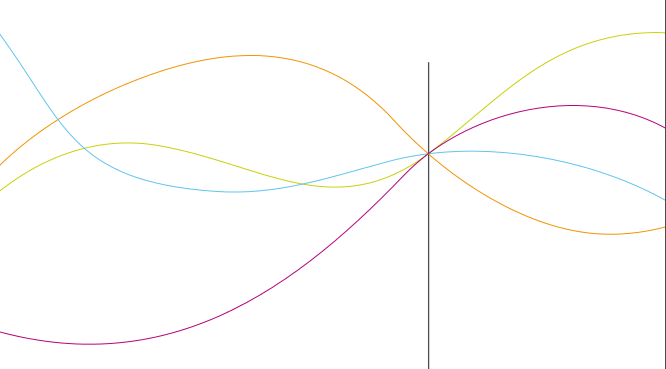
\includegraphics[scale=1]{images/bis1}}
    \put(-120,-50){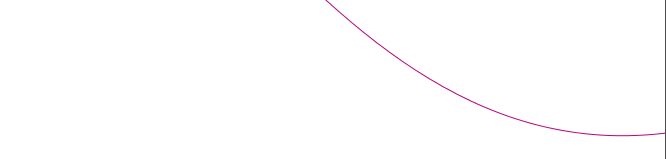
\includegraphics[scale=1]{images/bis2}}
    \put(0, -230){
      \begin{normalsize}
\begin{minipage}{15cm}
\textbf{Résumé :}\\
Le stage présenté dans ce rapport a été réalisé par Yicheng GAO dans la société Windeo Green Futur situé à Bruxelles de Belegique entre le 25 juin et le 31 Août 2012. Windeo Green futur est le leader européen en énergie renouvelable et maitrise de l'énergie, qui agit pour le développement des énergies renouvelables et apporte des solutions accessibles aux particuliers, entreprises et collectivités locales. Le stagiaire, en spécialité d'informatique, travaille au sein du département d'ingénierie, avec pour mission d’organiser et d’optimiser les opérations d’échange d’informations entre tout les acteurs éoliens de Windeo Green Futur.

Au cours de mon stage, je suis principalement intervenu sur la ma\^itrise d'ouvrage d'un projet d'application web. En temps que ma\^itrise d'ouvrage, j'ai du spécifier les besoins des clients internes, et établir la recette du application développée. A l'issue de ces 10 semaines de stage je peux dire que cette expérience a été très bénéfique pour moi. J'ai pu mettre en oeuvre mes compétences acquises lors de ma formation dans le département ASI et en acquérir de nouvelles.\\


\textbf{Abstract :}\\
The internship described in this report was conducted by Yicheng GAO in the society Windeo Green Future located in Brussels of Belegique between June 25 and August 31, 2012. Windeo Green future is the European leader in renewable energy and energy conservation, which devotes itself to the development of renewable energy and provides affordable solutions to individuals, companies and local authorities. The trainee, with a specialty of computer sciences, works in the engineering department, with the mission to organize and optimize operations between all actors of Windeo Green Future.

During my internship, I'm mainly occurred on the developpement of a web application project. During the developpement of this project, I have specified the needs of internal customers and established the recipe of developed application. At the end of the 10-week course I can say that this experience has been very beneficial for me. I could implement my skills acquired during my training in the ASI department and acquire new ones.


     \end{minipage}
      \end{normalsize}}
    \put(75, -550){
      \begin{normalsize}
        \begin{minipage}{10cm}
          \begin{tabular}{r}
            INSA de Rouen\\
            Avenue de l'Université - BP 08\\
            76801 Saint-Etienne-du-Rouvray Cedex\\
            Tél : 02 32 95 97 79\\
            Fax : 02 32 95 97 08\\
            https://asi.insa-rouen.fr\\
          \end{tabular}
        \end{minipage}
      \end{normalsize}}
    \put(320, -590){
\includegraphics[scale=1.4]{images/logoasi.png}}
    \put(170, -670){
\includegraphics[scale=0.5]{images/logoINSAdeRouenSlogan}}
  \end{picture}
}



\begin{document}

\pageINSA[twoside]

\pageDeGarde{Rapport de stage spécialité}{Mise en place d'une base \\de données réseau}
{ASI}{{GAO Yicheng}}{{ASI 4 -- 2011 - 2012}}

% \clearpage
\setcounter{tocdepth}{1}

\chapter*{Remerciements}
\addcontentsline{toc}{chapter}{Remerciements}	% permet de l'avoir dans le sommaire
Je souhaiterais tout d'abord remercier Nabila Chari et Loïc Pequignot, tous deux coordinateurs de la société Windeo Green futur, pour m'avoir accueilli chaleureusement au sein de leur équipe.\\

Je voudrais ensuite remercier mon tuteur de stage, Martina Pianta, pour toute l'aide qu'elle m'a apporté et tout le temps qu'elle m'a consacré pour mener à bien mon stage de spécialité. De plus, je souhaiterais remercier les autres membres de l'équipe technique du Windeo Green futur, Alexandre Gioffredy et Julie Grimes entre autres, pour avoir pris de leur temps pour répondre à mes questions et Mustapha Haddioui, pour ses explications sur l'utilisation de la plate-forme de wordpress.\\

Enfin, je voudrais remercier Guillaume Texier, stagaire aussi en EP 5 d'INSA de Rouen, sans qui ce stage ne se serait pas aussi bien déroulé. 


\tableofcontents


\chapter*{Glossaire}		
\addcontentsline{toc}{chapter}{Glossaire}	% permet de l'avoir dans le sommaire
\begin{description}
        \item[AJAX] \textsl{Asynchronous Javascript and XML}, est une manière de construire des applications Web et des sites web dynamiques basés sur diverses technologies Web ajoutées aux navigateurs dès 1995
        \item[API] \textsl{Application Program Interface}. Ensemble de conventions définissant de quelle manière un service peut-\^etre joint et utilisé par un logiciel
	\item[ASI] \textsl{Architecture des Systèmes d’Information}
        \item[CSV] \textsl{Comma-separated values}, est un format informatique ouvert représentant des données tabulaires sous forme de valeurs séparées par des virgules
	\item[EP] \textsl{Énergétique et Propulsion}
	\item[FTP] \textsl{File Transfer Protocol}, est un protocole de communication dédié à l’échange de fichiers sur un réseau
        \item[HTML] \textsl{HyperText Markup Language}. Langage permettant de construire des documents visualisables à l'aide de navigateur Web
        \item[HTTP] \textsl{HyperText Transfert Protocol}. Protocole de transfert de fichiers HTML à travers un réseau TCP/IP
        \item[INSA] \textsl{Institut National des Sciences Appliquées}
        \item[Javascript] Langage intialement proposé par Netscape qui permet d'inclure des fonctions au sein de pages HTML qui sont interprétées par le Navigateur
        \item[PHP]  \textsl{Hypertext Preprocessor}, est un langage de scripts libre principalement utilisé pour produire des pages Web dynamiques via un serveur HTTP
        \item[PIC] \textsl{Projet INSA Certifié}, projet industriel à mi-temps effectué par une équipe de 4-9 élèves-ingénieurs
        \item[SQL] \textsl{Structured Query Language}, est un langage informatique normalisé servant à effectuer des opérations sur des bases de données
        \item[XML] \textsl{eXtend Markup Language}. Langage extensible de balisage de documents, élaboré par le groupe de travail ERB (Editorial Review Board) du W3C (World Wide Web Consortium)

\end{description}

\chapter{Introduction}

Dans le cadre de ma scolarité au sein du département Architecture des Systèmes d'Information de l'Institut National des Sciences Appliquées de Rouen, il me fallait suivre une formation qui est consolidée par deux stages obligatoires. Ce rapport constitue une synthèse du travail effectué lors de mon stage de spécialité réalisé au sein de l'équipe Windeo Green Futur entre le 25 Juin et le 31 Août 2012 qui dure 10 semaines .\\

Le stage de spécialité permet de approfondir d'une part mon savoir-faire au sein de l'entreprise et permet de mettre en pratique d'autre part les connaissances acquises au cours de ma formation au sens du département ASI.\\

Ce rapport se divisera en 3 parties. Dans un premier temps, je donnerai une description de la société Windeo Green Futur, de ses objectifs et de quelques uns de ses outils. S'en suivra une présentation du travail effectué lors de ce stage de dix semaines. Enfin, je concluerai sur ce qui a été réalisé et sur les améliorations possibles à apporter. 


\chapter{Présentation de l'entreprise}
%% Présentation de l'entreprise et de l'endroit où vous vous situez [4-6 pages]

\section{Activité}

La société UINT développe et commercialise des circuits	électroniques fins, souples et autonomes embarqués dans	les cartes à puces. Les docteurs et ingénieurs au service d’UINT déploient leur forte expérience dans la recherche et le développement de l’électronique, de la sécurité des transactions et de la fabrication des cartes à puces, en maîtrisant tous les processus et cycles de vie des produits allant de la conception à la fabrication.\\

UINT a pour ambition d’être le leader mondial sur le marché des cartes à puces ISO dites actives (qui embarquent leur propre source d’énergie). En créant de la valeur ajoutée sur le support carte notamment via l’intégration de ses électroniques flexibles autonomes, UINT permet l’interactivité du porteur avec la carte et vice versa, offrant de nouveaux services disponibles 24h/24h qui vont révolutionner l’utilisation des cartes à puces avec leur environnement.\\

UINT a développé ses propres produits:\\

\begin{itemize}
\item \textit{U-GIFT} est une carte au format bancaire, embarquant une pile, un haut parleur et des diodes. Cette carte peut jouer de la musique et avoir des lumières qui scintillent. Cette carte est destinée au marché de l’affinitaire et de la carte cadeaux. Par exemple, une carte prépayée «joyeux anniversaire» qui peut jouer de la musique en plus de toutes les autres fonctions d’une carte cadeau «traditionnelle».
\item \textit{SPI} (Solution numérique d’impression sécurisée) est une solution logicielle et matérielle permettant de s’assurer que la personne qui imprime un document est la même que celle qui va récupérer les documents sur l’imprimante. Pour simplifier, pour récupérer les documents sur l’imprimante, la personne va devoir s’authentifier via un badge et un code pin.
\item \textit{uSecure} est une carte au format bancaire qui permet de contrôler l’émission d’une trame RF en appuyant sur un bouton. Il s’agit de la première carte RF contrôlée par l’utilisateur.
\end{itemize}


\subsection{Circuits flexibles}
UINT conçoit et développe ses circuits flexibles qui s’insèrent notamment dans des cartes au format bancaire ISO 7810. L’électronique utilisée dans les produits est choisie en fonction de ce critère de flexibilité ainsi que de leur faible consommation.

\begin{figure}[!htbp]
  \centering
    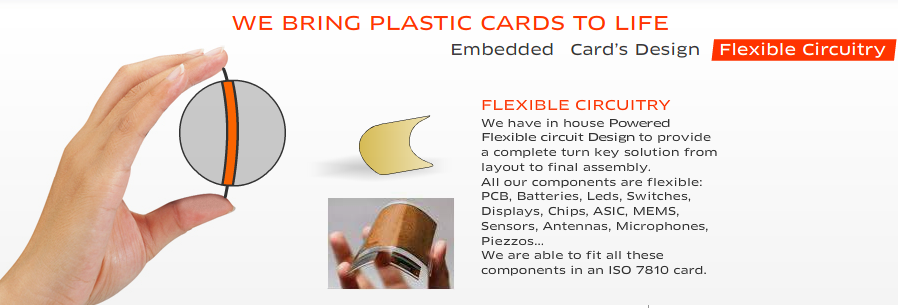
\includegraphics[scale=0.5]{images/flx}
  %\caption{Représentation schématique du cryptogramme}
  %\label{fig:auth}
\end{figure}


\subsection{Sécurité / Identification}

Que ce soit pour l’identification, l’authentification, le contrôle d’accès, le paiement ou tout autre service lié à la sécurité, l’expertise dans le domaine de la sécurité de notre équipe vous garantit une compréhension totale de votre projet.

\begin{figure}[!htbp]
  \centering
    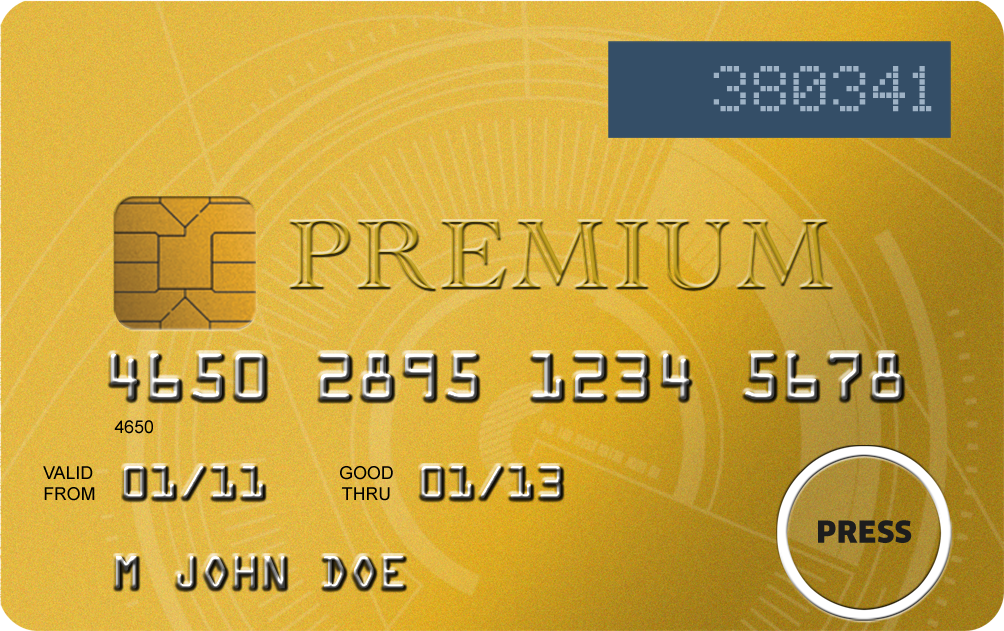
\includegraphics[scale=0.7]{images/pre}
  %\caption{Représentation schématique du cryptogramme}
  %\label{fig:auth}
\end{figure}

Voici quelques exemples de produits phares et voies de développement envisagées:\\

\begin{itemize}
\item Jeu: carte de jeu prépayée
\item Santé: auto contrôle de paramètres physiologiques (pouls, température…)
\item Sécurité: affichage de mot de passe dynamique ; contrôle de l’émission de signature RF, acoustique, biométrie
\item Marketing: carte musicale, à lumière, à écran…
\item Logistique: traçabilité, surveillance de température, capteurs…\\
\end{itemize}

Concernant les modèles de revenus de la société, ces derniers sont variables suivant les projets. Lorsqu’UINT réalise de la R\&D pour ses clients en vue de la fabrication de leurs produits, la société se rémunère sur cette R\&D et bénéficie de royalties ou licences sur les produits. Lorsqu’il s’agit de ses propres produits, par exemple la U-GIFT Card, UINT démarche les grands noms des distributeurs ou émetteurs de cartes cadeaux / fidélité pour mettre la U-GIFT Card dans leur catalogue. Dans ce cas, UINT personnalise la carte (visuel, musique) à la demande du client qui, lui, vendra la carte en «boutique».

\section{Stratégie}

La R\&D est au cœur de l’activité de la société. Sur les 8 salariés, 7 ont une formation de type technique (électronique ou informatique) dont 3 docteurs et 2 ingénieurs. Il est à noter que deux des produits conçus par UINT ont reçu une certification Mastercard.\\ 

Sur le territoire national, UINT n’a aucune concurrence. Au plan international, bien qu’il y ait des sociétés proposant des produits «cartes» avec de l’électronique flexible, aucune ne se positionne comme UINT avec un portfolio de produits aussi variés. Hormis UINT, à notre connaissance, la concurrence ne conçoit et ne produit que des cartes avec un afficheur dans le domaine de la sécurité.\\

Come abordé précédemment, UINT maitrise la conception de circuits flexibles ainsi que la gestion de la faible consommation des composants électroniques.\\

La société UINT a reçu «L’Électron d’Or de la meilleure Start-Up 2010» lors de la cérémonie qui s’est tenue au siège parisien de la FIEEC (Fédération des Industries Électriques, Électroniques et de Communication), le 16 juin 2010. Ce prix est remis par le magazine ÉlectroniqueS et le sponsor RS parmi les 12 lauréats de cette 13ème édition. Les nominés sont des entreprises et des grands groupes nationaux et internationaux (France, Etats-Unis, Allemagne, Royaume-Uni, Norvège, Japon…) repérés par la rédaction du journal à travers l’actualité de leur activité ou de leurs projets. Un jury expert comptant des professionnels du secteur, des consultants et des membres de la rédaction du journal ElectroniqueS est chargé de l’attribution des prix.\\

La société UINT a reçu le prix «de l’innovation à l’internationale 2010» lors du 5ème forum de l’international à Evry le 9 décembre 2010. Ce prix a été décerné par la CGPME 91 et la CCI Essonne.\\

Enfin, la société s’est tournée ces derniers mois vers la Chine en vue d’établir des partenariats technologiques, commerciaux et avec des distributeurs. Depuis le 4 janvier 2011, elle a signé deux contrats avec un partenaire technologique (fabrication de carte) et un distributeur.\\

UINT vient de créer sa propre usine d’hybridation (soudage des composants électroniques au circuit flexible), afin de réduire les coûts de fabrication et augmenter ainsi sa marge. UINT souhaite également agrandir son équipe d’ingénieurs en électronique afin de toujours concevoir de nouveaux produits innovants.

\section{Ressources humaines}

A ce jour, UINT est composée de 8 salariés. UINT fait principalement de la R\&D. Sur les 8 salariés, 7 ont une formation de type technique (électronique ou informatique) dont 2 docteurs et 5 ingénieurs.\\

Ce bilan est antérieur à l’ouverture des Laboratoires sur le site de Limoges et qui doit conduire à l’ouverture d’une vingtaine de postes d’ici fin 2014.

\begin{figure}[!htbp]
  \centering
    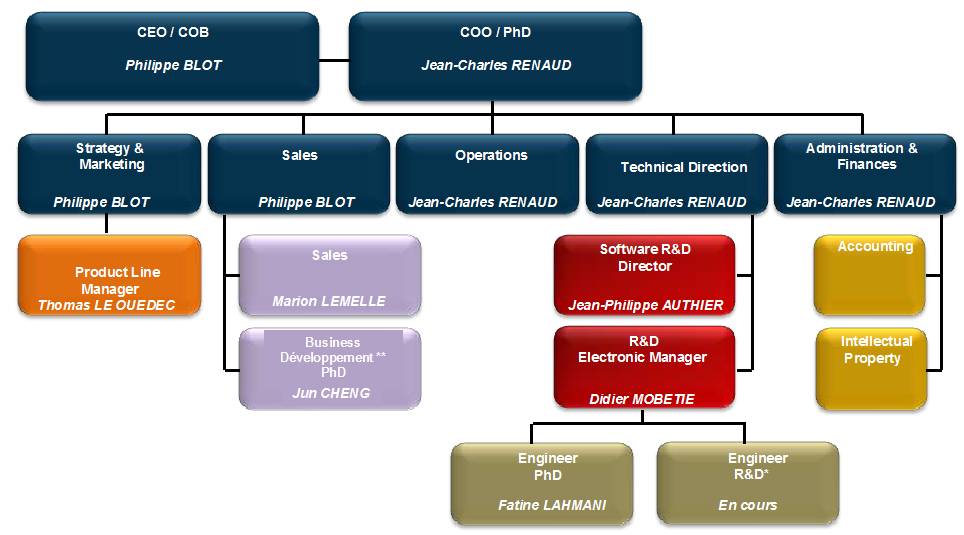
\includegraphics[scale=0.6]{images/rh}
  %\caption{Représentation schématique du cryptogramme}
  %\label{fig:auth}
\end{figure}

\section{Ressources technologiques}

\subsection{Savoir faire et technologies maitrisées}

\begin{itemize}
\item UINT maitrise la conception de circuits fins et flexibles ainsi que la gestion de la faible consommation des composants électroniques.
\item UINT maitrise l'hybridation des composants électroniques sur circuit flexible
\item UINT invente, conçoit, développe et distribue des solutions de cartes multifonctions avec des microprocesseurs sécurisés et autonomes.
\item UINT conçoit et développe des solutions pour authentifier des utilisateurs lors d’échanges sécurisés.
\end{itemize}

\subsection{En termes de protection industrielle, elle possède des brevets}

\begin{itemize}
\item \textit{WO2011067543:} activation et indication d’un champ RF sur un dispositif comprenant une puce
\item \textit{PCT / FR 2010 / 052767:} carte à puce multi-applicatifs avec validation biométrique
\item \textit{FR 2953619:} dispositif électronique (jeton) téléphonique
\end{itemize}

\subsection{Certifications acquises}

A l’heure actuelle, la société UINT ne possède pas de certification, néanmoins deux de ses produits ont reçu une certification Mastercard.




\chapter{Présentation du sujet du stage}
%% Présentation du sujet du stage [1-2 pages]

Le stagiaire, en spécialité informatique, travaille au sein du département d'ingénierie, avec pour mission d’organiser et d’optimiser les opérations d’échange d’informations entre tous les acteurs éoliens de Windeo.\\

Dans un premier temps, le stagiaire se concentrera sur la mise en place d’un système dynamique permettant d’améliorer la base de données interne, dont l'objectif est d'adapter l’espace intranet sur le site web, afin de permettre la collecte des informations et un export vers sur une base de donnée (Access, FilemakerPro ou autre) pour qu’elles constituent un récapitulatif des opérations d’intervention d’installation et de maintenance sur l’ensemble du parc éolien.\\

En ce moment, le site intranet est supporté par Wordpress (un CMS) et GoogleDoc (un outil Google), qui est figuré ci-dessous. Les clients doivent remplir plusieurs sous-formulaires (formulaire pour le mât, la turbine, etc.) sur le site de constructeur et de Windeo Green Futur, ce qui entraîne des informations redondantes et une complexité de remplissage.\\

\begin{figure}[!htbp]
  \centering
    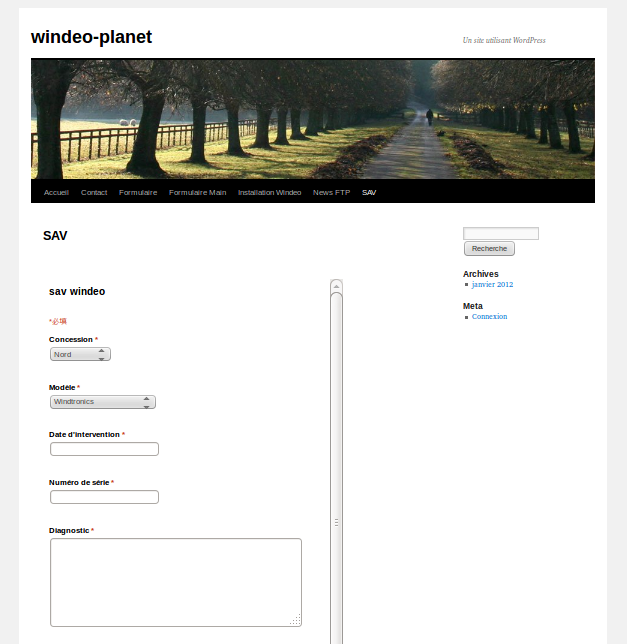
\includegraphics[scale=0.3]{images/web-old}
  \caption{Formulaire avec l'outil \texttt{GoogleDoc}}
  %\label{fig:auth}
\end{figure}

\begin{figure}[!htbp]
  \centering
    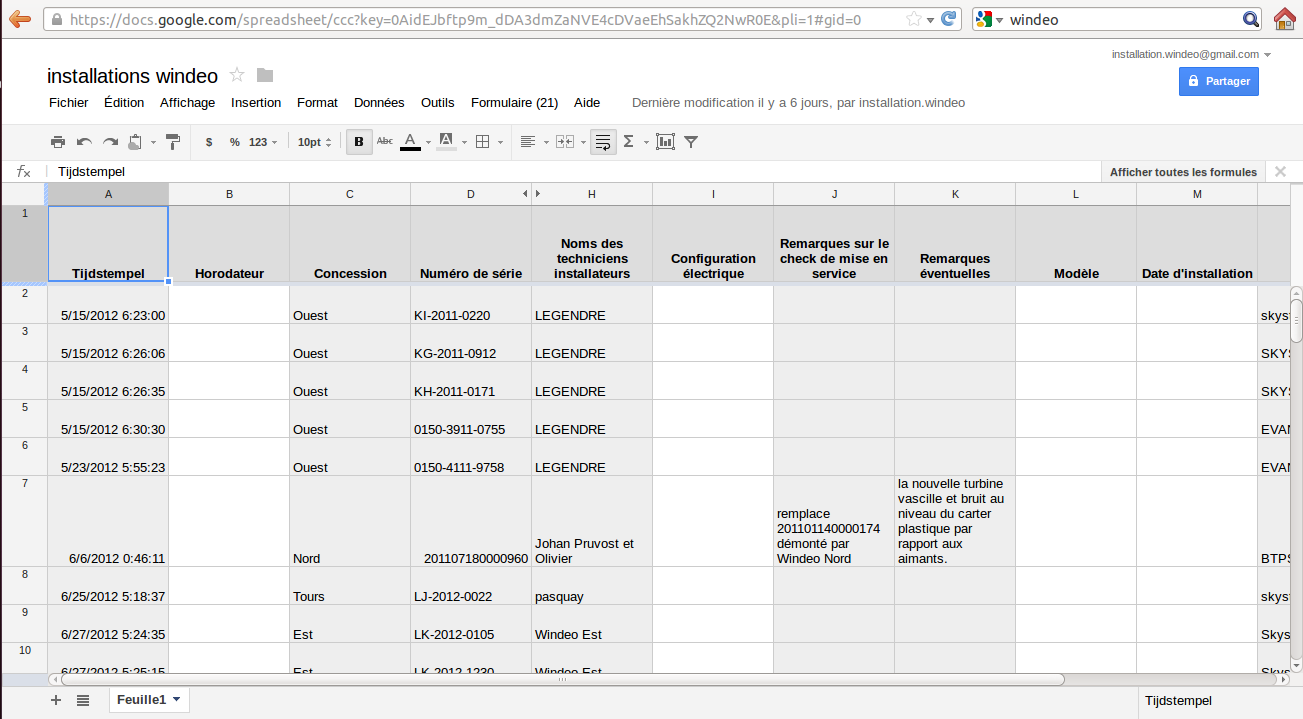
\includegraphics[scale=0.3]{images/data-old}
  \caption{Les données envoyées par \texttt{GoogleDoc}}
  %\label{fig:auth}
\end{figure}

\newpage
Une deuxième partie du stage, consistera à faciliter l’échange d’information et garantir une homogénéité des fichiers utilisés par le département d’ingénierie et les équipes techniques. La base de données repose actuellement et reposera idéalement sur un serveur File Transfert Protocol, mais tout autre système qui sera jugé intéressant par le stagiaire et l’équipe sera pris en compte. Une procédure de synchronisation des données émises et rectifiées par les participants au réseau au fur et à mesure devra être mise en place. (Procédure « Dropbox »).\\


\chapter{Le travail effectué}
%% Le travail effectué [10-20 pages]
%% Vous devez montrer les points conceptuels et techniques importants :
%% Étude du cahier des charges
%% Propositions et critiques de solutions
%% Description complète de la solution choisie
%% Mise en oeuvre
%% Résultats obtenus (critique)

\section{Étude du cahier des charges}
\label{CDC}
\subsection{L’espace intranet \texttt{wordpress}}
Pour la première partie du stage concernant l’espace intranet, l’utilisation du \texttt{wordpress} et \texttt{GoogleDoc} fonctionne bien, le formulaire est généré automatiquement par \texttt{GoogleDoc} et les données sont envoyées vers le compte \texttt{Google} qui les a déjà enregistrées. Mais il y a quelques inconvénients supplémentaires à ceux présentés dans le sujet de stage si on utilise cette méthode:\\

\begin{itemize} 
\item Les données ne peuvent être visualisées qu'en format XSL dans un compte \texttt{GoogleDoc}
\item Il faut créer un compte Google public 
\item Le formulaire généré par \texttt{GoogleDoc} est trop simple, et n'a pas de fonctionnalités avancées \\
\end{itemize}

Donc il faut chercher une autre méthode pour présenter le formulaire et un moyen plus efficace pour exporter les données envoyées par les clients.  

\subsection{L’échange d’information avec FTP}

Pour la deuxième partie du stage concernant l’échange d’information et l'homogénéité des fichiers, le transfert des fichiers internes est supporté actuellement par un serveur FTP, mais toutes les opérations pour les fichiers doivent être faites manuellement, on a besoin d'ajouter une procédure de synchronisation des fichiers entre les machines locales et les machines à distances.\\

L'objectif est de metrre en place un système figuré ci-dessous: Les administrateurs ont les droits R\&W, c'est-à-dire lire et écrire des fichiers dans le serveur, les clients ont le droit W seulement, et s'ils veulent modifier les fichiers sur FTP, il faut envoyer un mail de notification aux administrateurs.\\

Les fichiers sont synchronisés entre un serveur local et le serveur FTP, les fichiers sur le serveur local sont synchronisés partiellement avec les ordinateurs des administrateurs.

\begin{figure}[!htbp]
  \centering
    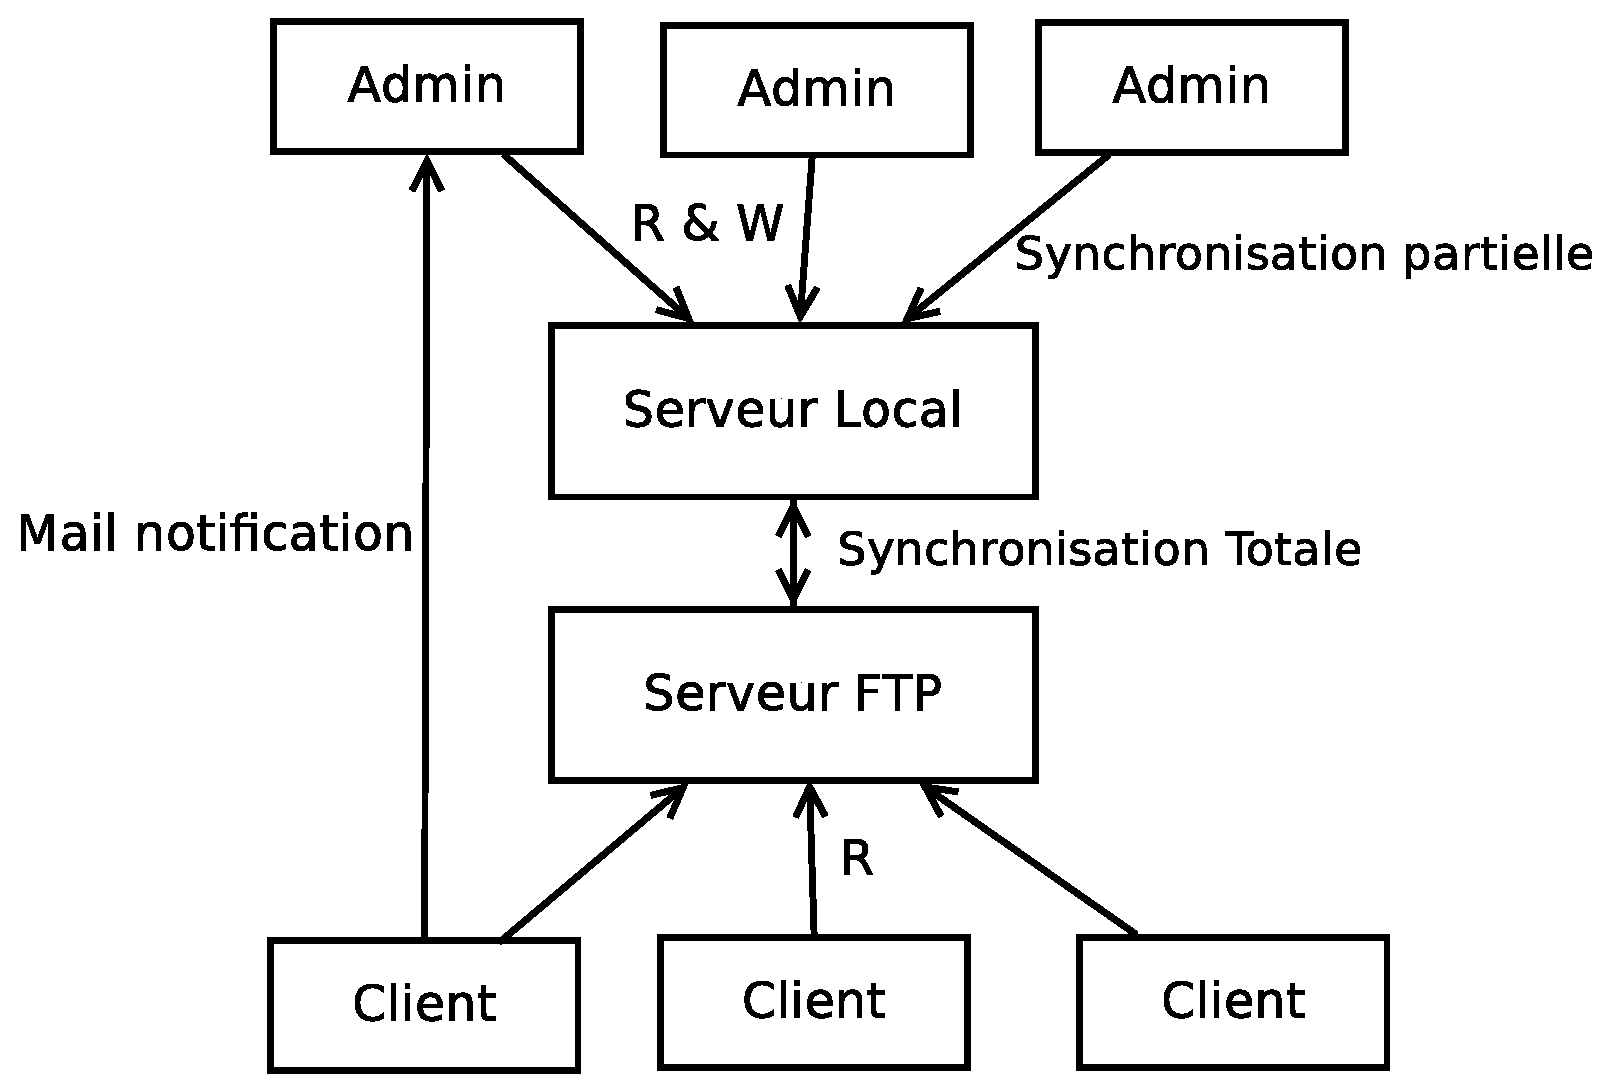
\includegraphics[scale=0.5]{images/FTP}
  \caption{L'objectif d'utilisation du FTP}
  %\label{fig:auth}
\end{figure} 
%%%%%%%%%%%%%%%%%%%%%%%%%%%%%%%%%%%%%%%%%%%%%%%%%%%%%%%%%%%%%%%%%%%%%%%%%%%%%%%%%%%%%%%%%%%%%%%%
\section{Propositions des solutions possibles}

  \subsection{L’espace intranet \texttt{wordpress}}
Pour l'espace intranet, je conseille de conserver le modèle wordpress mais de remplacer l'outil \texttt{GoogleDoc} par une extension wordpress qui s'appelle \texttt{WordPress Form Manager}, qui est destinée pour générer les formulaires professionnels.

     \subsubsection{Wordpress}


\begin{wrapfigure}[]{r}{70mm}
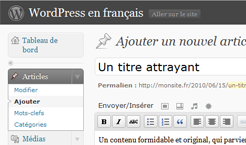
\includegraphics[scale=0.8]{images/wordpress.png}
\caption{Page d'adminisrtation de \texttt{wordpress}}
\end{wrapfigure}


WordPress est un système de gestion de contenu (CMS) qui permet de créer et gérer facilement l'ensemble d'un site web ou simplement un blog. Gratuit et libre, WordPress est personnalisable grâce à de nombreux thèmes et plugins(extensions).\\

En outre, il existe une solide communauté à travers le monde entier.\\

WordPress constitue le nec plus ultra en matière de plates-formes sémantiques de publication personnelle, alliant esthétique, standards du Web et ergonomie. Gratuit, WordPress n ’en est pas moins inestimable. Sous licence GPLv2+, cet outil est libre de droits.\\

Plus simplement, WordPress est ce qu’il nous faut si on veut avancer au moyen d’un système de gestion de contenu.\\





    \subsubsection{Les plugins du \texttt{wordpress}}
Les plugins permettent d'étendre les fonctionnalités de wordpress. Les plugins du wordPress peut s'étendre de faire presque tout ce qu'on peut imaginer, ils sont généralement crées par tout le monde, gratuits, et open-source. Dans notre site, on utilise quelques plugins:\\

\begin{itemize}
\item WordPress Form Manager
\item Database Browser
\item Configure SMTP
\item Code Insert Manager
\item etc.
\end{itemize}

    \paragraph{WordPress Form Manager}

WordPress Form Manager est un gestionnaire de formulaires qui stocke dans une table les informations fournies par les utilisateurs. Le plugin permet la gestion de fichiers joints et de captchas. La création de formulaires est très intuitive et une documentation très riche existe. Dans les plus: un affichage de formulaires interactif. Par exemple, on peut demander à afficher un champ texte uniquement lorsque l’utilisateur aura coché un certain bouton plus haut dans le formulaire. C’est une fonction impressionnante qui permet de complexifier sans lourdeur un formulaire. Dans les moins: la gestion de présentation des mails envoyés est vraiment très compliquée. Par défaut, les contenus des champs sont présentés sous forme de liste.\\
  
Form Manager est un outil pour créer des formulaires pour collecter et télécharger des données de visiteurs du site WordPress. Les formulaires sont ajoutés à des articles ou des pages en utilisant un shortcode simple, ou peut être ajouté au thème avec une API simple.\\

\begin{wrapfigure}[]{r}{80mm}
\centering
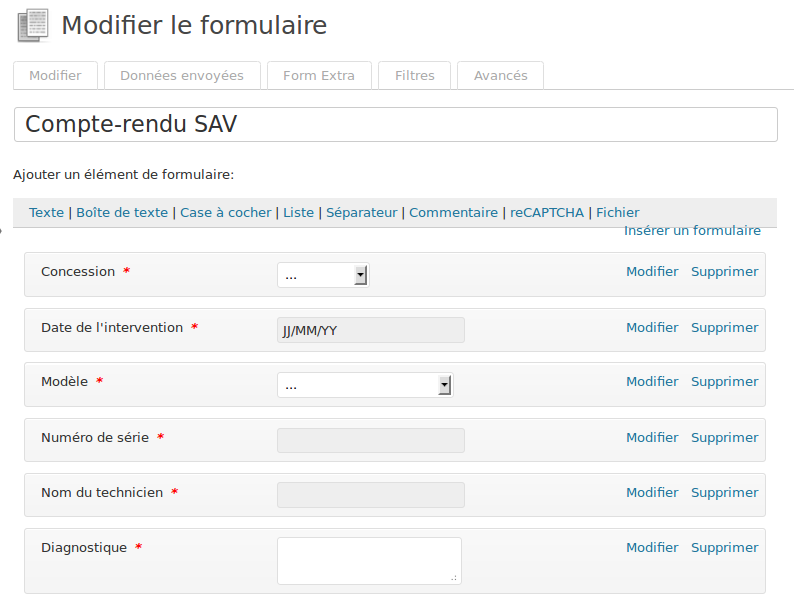
\includegraphics[scale=0.25]{images/formManager}
\caption{Page d'adminisrtation de plugin \texttt{Form Manager}}
\end{wrapfigure}

Les fonctionnalités:
\begin{itemize}
\item validation
\item champs requis
\item remerciements personnalisés
\item notifications par email
\item templates d'affichage des formulaires\\
\end{itemize}

Types de champs supportés:
\begin{itemize}
\item texte
\item zone de texte
\item liste déroulante
\item bouton radio
\item cases à cocher
\item sélection multiple
\item téléchargement
\item reCAPTCHA
\end{itemize}

    \paragraph{Database Browser}
Database Browser est un gestionnaire de base de données qui permet de connecter à notre serveur SQL, Oracle ou ODBC, d'en modifier les données, de les tester avec des scripts SQL mais également d'exporter et d'imprimer les données. L'application supporte un nombre illimité de connexions et permet de naviguer dans les tables rapidement et facilement. Un outil de recherche, un historique, un module d'exécution des fichiers LOG et d'autres options sont également disponibles.

  \subsection{L’échange d’information avec FTP}
  \label{infoFTP}
Avec le cahier de charge ci-dessus, je propose de concevoir une application Web qui a pour objectif de réaliser les opérations concernant le FTP, par exemple:\\

\begin{itemize}
\item On peut se connecter avec deux comptes différents, un compte administrateur et un compte utilisateur
\item Tous les utilisateurs peuvent visualiser les données dans le serveur FTP
\item Il y a une liste de demandes de changement des fichiers donnée par le client, si on se connecte avec le compte administrateur, on peut les autoriser ou les refuser\\
\end{itemize}

Pour la procédure de synchronisation, il y en a pas mal de logiciels qui existent déjà.

%%%%%%%%%%%%%%%%%%%%%%%%%%%%%%%%%%%%%%%%%%%%%%%%%%%%%%%%%%%%%%%%%%%%%%%%%%%%%%%%%%%%%%%%%%%%%%%%
\section{Mise en oeuvre}
  \subsection{Phrase de préparation}
Les exigences minimales pour exécuter WordPress sont:

\begin{itemize}
\item PHP version 5.2.4 
\item MySQL version 5.0 \\
\end{itemize}

Dans ce cas, on a besoin:
\begin{itemize}
\item de l’accès d'un serveur FTP
\item d'un logiciel puissant permettant de manipuler les fichiers sur le serveur FTP 
\item d'un système d'exploitation de type linux
\item de l'environnement PHP
\item de l'environnement base de donnée MySQL
\item de la ré-installation du \texttt{wordpress}
\item d'un logiciel pour manipuler la base de donnée (\texttt{phpMyAdmin} par exemple)
\end{itemize}

     \subsubsection{connecter au serveur FTP} 
Le DSI m'a donné un compte pour accéder au serveur FTP de la société, qui a les droits d'écrire et de modifier les fichiers.\\

Pour la manipulation des fichiers dans le FTP, il a recommandé le logiciel \texttt{FileZilla}.\\

FileZilla est un client FTP. Un logiciel libre qui permet de charger ou télécharger les fichiers sur un serveur. Il possède une interface utilisateur graphique intuitive. On choisie ce logiciel pour les raisons suivants:\\

\begin{itemize}
\item logiciel Open-source
\item Rapide et fiable, facile à utiliser
\item Multi-plateforme. Fonctionne sur Windows, Linux, BSD, Mac OS X et plus. C'est importante parce que les personnes dans l'équipe utilisent les différents types de OS.
\item Disponible dans de nombreuses langues, car les clients viennent des differents pays
\end{itemize}


     \subsubsection{Installation l'OS Ubuntu}
À l'INSA, on utilise beaucoup le système d'exploitation de type linux, Ubuntu par exemple.
Ubuntu est un système d’exploitation libre commandité par la société Canonical et c'est une marque déposée par cette même société.\\

Fondé sur la distribution Linux Debian et utilisant le bureau Unity, Ubuntu se veut « convivial, intuitif et sûr ». Il est constitué de logiciels libres, est disponible gratuitement y compris pour les entreprises, et bénéficie d'une nouvelle version tous les six mois.\\

Avec une utilisation globale estimée à plus de 25 millions d'utilisateurs, il est principalement conçu pour une utilisation sur des ordinateurs personnels (portables et fixes), bien que d'autres versions consacrées aux netbooks et aux serveurs existent aussi. \\

     \subsubsection{Installation d'environnement PHP}
Pour faire fonctionner \texttt{wordpress}, il faut un environnement PHP sur le serveur.
Je l'ai installé suivant les instructions du cours Technologie Web encadré par M.Alexandre Pauchet:\\
 
\begin{itemize}
\item Récupérer des sources dans \url{http://www.apache.org} et \url{http://www.php.net} et déposer les 2 archives dans \texttt{<chemin>/srcweb}
\item Décompression des sources
\item Configuration de la compilation
\item Compilation
\item Test d'Apache et du module PHP dans Apache
\end{itemize}

     \subsubsection{Installation de la base de donnée}
     \label{database}
Si on utilise le CMS \texttt{wordpress}, il faut une base de données associée à ce site, pour ce faire, j'ai installé la base de données avec \texttt{MySQL}. On peut créer un tableau facilement avec quelques lignes de commande.

     \subsubsection{Mise en place de Wordpress}
\begin{itemize}
\item[Étape 1:]Téléchargez et décompressez WordPress.
\item[Étape 2:]Créez une base de données pour WordPress sur le serveur Web(Voir \ref{database}), de sorte que MySQL ait tous les privilèges en accès et en modification.
\item[Étape 3:]Ouvrez le fichier \texttt{wp-config.php} dans l'éditeur de texte et complétez les informations de la base de données (et le langage utilisé par le blog si nécessaire).
\item[Étape 4:]Déposez les fichiers de WordPress à l'emplacement désiré sur votre serveur Web :
\item[Étape 5:]Comme on a téléchargé la version anglaise de WordPress, vous devez copier les fichiers de traduction fr\_FR.mo et continents-cities-fr\_FR.mo (correspondants à la version de WordPress installée) dans le sous-dossier \texttt{wp-content/languages}. Ensuite, modifiez le fichier \texttt{wp-config.php} pour avoir define ('WPLANG', 'fr\_FR')
\item[Étape 6:]Lancer le script d'installation de WordPress en ouvrant \texttt{wp-admin/install.php} dans votre navigateur Web préféré.
\end{itemize}    
 
     \subsubsection{Clés secrètes pour la base de données}    
Une clé secrète qui rend le site plus difficile à pirater et plus difficile à casser en ajoutant des éléments aléatoires pour le mot de passe.\\

En termes simples, une clé secrète est un mot de passe avec des éléments qui font qu'il est plus difficile de générer suffisamment d'options pour percer les barrières de sécurité. Un mot de passe comme "mot de passe" ou "test" est simple et se brisent facilement. Une aléatoire, imprévisible mot de passe tels que "88a7da62429ba6ad3cb3c76a09641fc" prend des années à venir avec la bonne combinaison.\\

Un exemple d'utilisation des clés secrètes:\footnote{extrait du tutoriel \texttt{Wordpress}}
\begin{verbatim}
define('AUTH_KEY',         't`DK%X:>xy|e-Z(BXb/f(Ur`8#~UzUQG-^_C');
define('SECURE_AUTH_KEY',  'D&ovlU#|CvJ##uNq}bel+^MFtT&.b9{UvR]g');
define('LOGGED_IN_KEY',    'MGKi8Br(&{H*~&0s;{k0<S(O:+f#WM+q|npJ');
define('NONCE_KEY',        'FIsAsXJKL5ZlQo)iD-pt??eUbdc{_Cn<4!d~');
define('AUTH_SALT',        '7T-!^i!0,w)L#JK@pc2{8XE[DenYI^BVf{L:');
define('SECURE_AUTH_SALT', 'I6`V|mDZq21-J|ihb u^q0F }F_NUcy`l,=o');
define('LOGGED_IN_SALT',   'w<$4c$Hmd%/*]`Oom>(hdXW|0M=X={we6;Mp');
define('NONCE_SALT',       'a|#h{c5|P &xWs4IZ20c2&%4!c(/uG}W:mAv');
\end{verbatim}



  \subsection{Mise en place du formulaire}

\begin{wrapfigure}[]{r}{80mm}
\centering
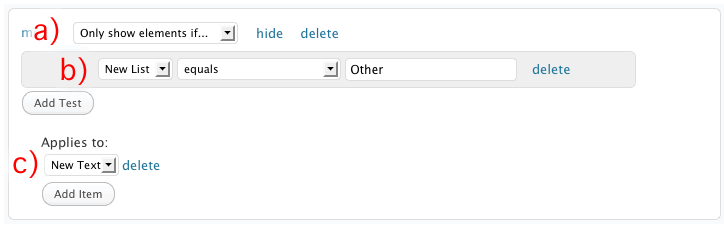
\includegraphics[scale=0.3]{images/form}
\caption{Un filtre du formulaire réalisé en \texttt{AJAX}}
\end{wrapfigure}

J'ai établi les formulaires en fonction des exigences des fournisseurs du Windeo Green futur, 
l’objectif des formulaires est de collecter les informations des différents turbines, mais chaque 
turbine a un type d'informations différent, donc il faut résumer les différents types de turbines 
et les mettre dans un seul formulaire.\\

Selon le type de turbine choisi, les lignes de formulaire apparaissent en fonction du choix de la turbine, pour ce faire, j'ai essayé de le faire avec AJAX, 
mais je n'y suis pas arrivé (explication en \ref{code}), donc on a cherché un autre plugin qui peut ajouter un filtre dans le formulaire comme figuré à droite. 

  \subsection{Mise en place d'une fonction d'authentification}

D'après la demande des personnes de la centrale d'achat, il faut ajouter une fonction d'authentification sur le wordpress, c'est-à-dire un mot de passe requis pour accéder aux pages du site. Mais malheureusement, le wordpress ne supporte pas cette fonctionnalité par défaut, donc il faut l'ajouter à la main.\\

D'abord, j'ai ajouté un fichier \texttt{login.php} dans le répertoire principal du site, qui est un script d'affichage, pour lire le mot de passe donné par l'utilisateur.\\

J'ai ensuite ajouté une partie de code PHP (Voir dans Annexe) dans le fichier \texttt{header.php}, qui utilise le concept \texttt{SESSION} dans PHP.\\

Les résultats sont figurés ci-dessous:\\

\begin{center}
\begin{tabular}{c c}
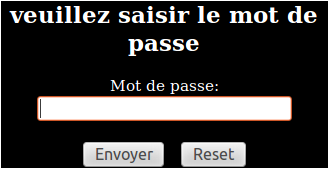
\includegraphics[scale=0.7]{images/auth1} & 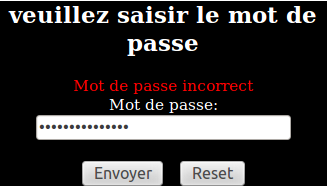
\includegraphics[scale=0.64]{images/auth2} \\
Page d'authentification & Page d'authentification en cas d'échec
\end{tabular}
\end{center}
%%%%%%%%%%%%%%%%%%%%%%%%%%%%%%%%%%%%%%%%%%%%%%%%%%%%%%%%%%%%%%%%%%%%%%%%%%%%%%%%%%%%%%%%%%%%%%%%
\section{Problèmes rencontrés}

\subsection{Exporter les données de wordpress}
\label{donnee}
Si on veut exporter les données du formulaire en format \texttt{.csv} avec le plugin \texttt{Database browser}, il apparaît un avertissement listé ci-dessous:\\
 
\begin{verbatim}
Warning: Cannot modify header information - 
headers already sent in /var/www/vhosts/windeo-planet.com/httpdocs/www/
wordpress/wp-content/plugins/wordpress-form-manager/getcsv.php on line 36

Warning: Cannot modify header information - 
headers already sent in /var/www/vhosts/windeo-planet.com/httpdocs/www/
wordpress/wp-content/plugins/wordpress-form-manager/getcsv.php on line 37

Warning: Cannot modify header information - 
headers already sent in /var/www/vhosts/windeo-planet.com/httpdocs/www/
wordpress/wp-content/plugins/wordpress-form-manager/getcsv.php on line 38

Warning: Cannot modify header information - 
headers already sent in /var/www/vhosts/windeo-planet.com/httpdocs/www/
wordpress/wp-content/plugins/wordpress-form-manager/getcsv.php on line 39
\end{verbatim}

qui concerne cette partie(lignes 36-39) du fichier \texttt{getcsv.php}:
\begin{verbatim}
header("Content-type: application/csv");
header("Content-Disposition: attachment; 
        filename=\"".$formInfo['title'].".csv\"");
header("Pragma: no-cache");
header("Expires: 0");
\end{verbatim}

Après la recherche sur Internet, cela est souvent dû à des lignes blanches ou espaces au début d'un fichier \texttt{.php}, ceux-ci doivent impérativement commencer par \texttt{<?php} et rien d'autre.
Après la vérification des fichiers concernés, je ne vois aucune ligne blanche ou espace avant \texttt{<?php}. Par ailleurs,  
dans wordpress, on ne peut pas toucher les fichiers générés (explication dans \ref{code}). Je suppose alors c'est peut-être à cause d'un conflit des plugins, mais je ne peux pas désactiver les autres plugins, ni faire de modifications, 
donc je propose deux solutions possibles:\\

\begin{itemize}
\item Désactiver l'avertissement du PHP
\item Chercher une autre méthode pour exporter les données \\
\end{itemize}

Finalement, j'ai choisi la mise en place de l'outil \texttt{phpMyAdmin} pour faire la gestion de la base de données:\\

\begin{wrapfigure}[]{r}{95mm}
\centering
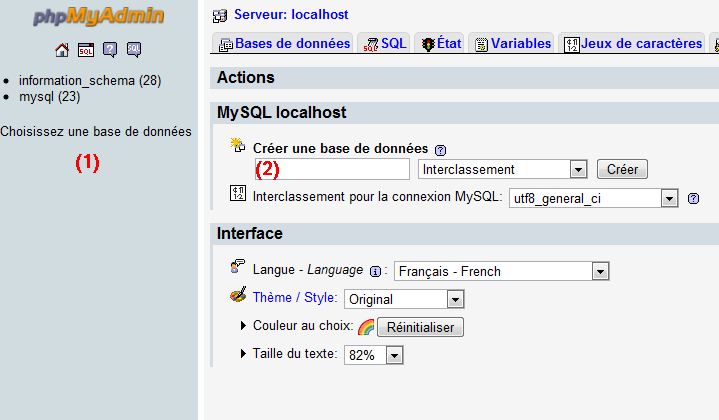
\includegraphics[scale=0.4]{images/phpmyadmin}
\caption{Capture d'écran \texttt{PhpMyAdmin}}
\end{wrapfigure}

phpMyAdmin (PMA) est une application Web de gestion pour les systèmes de gestion de base de données MySQL réalisée en PHP et distribuée sous licence GNU GPL.\\

Il s'agit de l'une des plus célèbres interfaces pour gérer une base de données MySQL sur un serveur PHP. De nombreux hébergeurs, qu'ils soient gratuits ou payants, le proposent ce qui permet à l'utilisateur de ne pas avoir à l'installer.\\

\subsection{Personnalisation du wordpress}
\label{code}
J'ai proposé de faire la personnalisation du \texttt{wordpress}, par exemple, d'ajouter les codes PHP dans une page qui existe déjà, faire le changement de mise en pages du formulaire, etc. Car la fonctionnalité du \texttt{wordpress} n'est pas suffisante, mais malheureusement ce n'est pas possible à ce moment-là. \\

En effet, on voulait bien ajouter une fonction \texttt{AJAX} pour faire un formulaire dynamique, mais je n'ai pas trouvé le fichier \texttt{.php} concernant ce formulaire. Après l'étude du wordpress plus profondément, j'ai trouvé le mécanisme de ce CSM: Il n'existe pas de fichiers réels pour chaque page, mais ils sont générés par les modèles définis par les fichiers \texttt{.php} du wordpress et par la base de données. Par exemple, si on veut faire l'affichage des données en format \texttt{csv} (présenté dans \ref{donnee}), le wordpress appelle le fichier \texttt{getcsv.php} dans dossier du plugin et les données stockées dans la base de donnée.\\

De cette façon, on ne peut pas faire la personnalisation des pages, sauf si on change les codes sources du plugin, ou si on remplace les plugins par un autre plugin. 

\subsection{Notifications par mail}

On a besoin d'envoyer un mail si un formulaire est rempli, mais si on fait un test, il y a toujours une erreur listée ci-dessous:

\begin{verbatim}
An error was encountered while trying to send the test e-mail.
SMTP Error: Could not connect to SMTP host.
\end{verbatim}

J'ai vérifié que les configurations de boîte mail et les portes des SMTP étaient correctes, mais l'ordinateur ne peut toujours pas se connecter au serveur SMTP. Après beaucoup de recherche sur Internet, j'ai vu une autre raison éventuelle: le serveur a interdit la fonction \texttt{fsockopen()} qui concerne la fonctionnalité de mail, on peut le remplacer par \texttt{pfsockopen()}, mais malheureusement, après la changement, ça ne fonctionnait toujours pas.\\

J'ai pensé ensuite que cela était peut-être dû aux configurations du serveur du site, donc j'ai envoyé un mail à la DSI pour demander de vérifier les configurations du SMTP sur le serveur, et la DSI m'a repondu que les portes de SMTP étaient fermées par défaut dans le serveur, après ce changement, cela a parfaitement fonctionné.

%%%%%%%%%%%%%%%%%%%%%%%%%%%%%%%%%%%%%%%%%%%%%%%%%%%%%%%%%%%%%%%%%%%%%%%%%%%%%%%%%%%%%%%%%%%%%%%%
\section{Résultats obtenus}
Enfin, j'ai mis en place 4 formulaires pour la société Windeo Green Futur:\\

\begin{itemize}
\item Formulaire d’installation
\item Formulaire maintenance ordinaire
\item Formulaire SAV
\item Formulaire type ARE\\
\end{itemize} 

C'est un exemple des formulaires qu'on a établi durant mon stage:

\begin{figure}[!htbp]
  \centering
    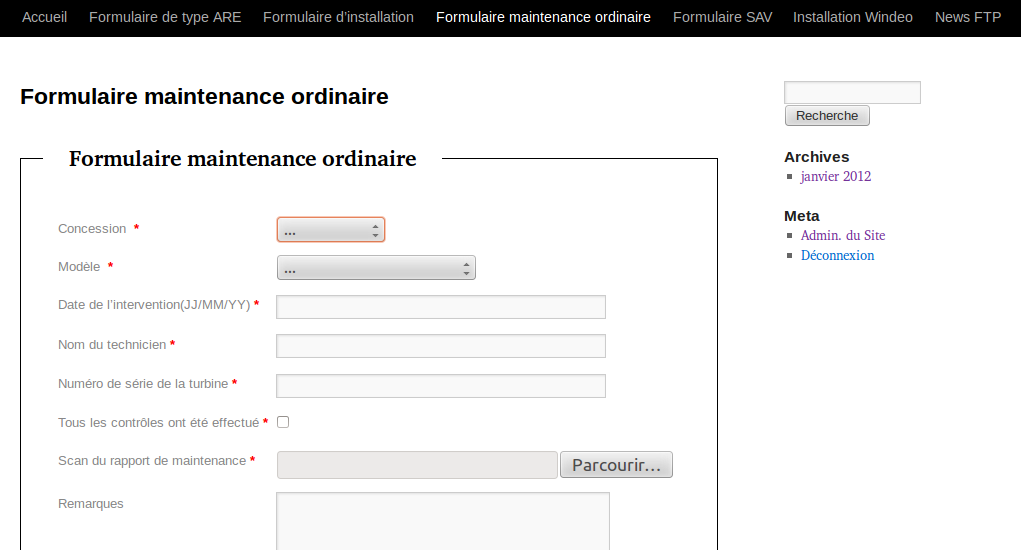
\includegraphics[width=\textwidth]{images/resultat}
  \caption{Capture d'écran du formulaire maintenance ordinaire}
  %\label{fig:auth}
\end{figure}

\newpage

Pour la deuxième partie du stage, on n'a pas eu assez de temps pour concevoir l'application Web décrite dans le Cahier des charges, donc j'ai conseillé d'utiliser un logiciel existant qui s'appelle GoodSync et qui a les fonctionnalités suffisantes pour les manipulations des fichiers FTP.\\

GoodSync est un logiciel de synchronisation de fichiers et de sauvegarde de fichiers qui opère automatiquement les syncs entre PC de bureau, portables et disques externes.\\

\begin{figure}[!htbp]
\centering
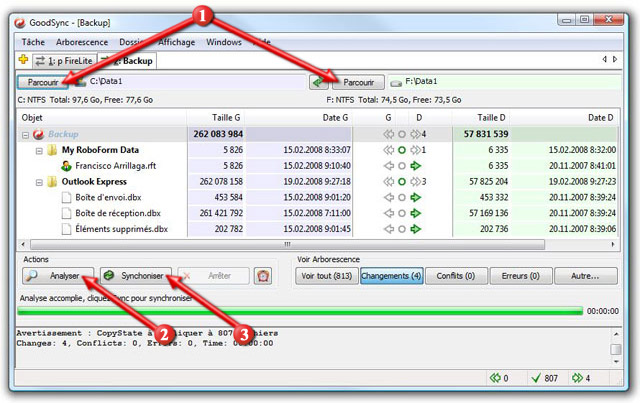
\includegraphics[scale=0.6]{images/Goodsync}
\caption{Logiciel \texttt{GoodSync}}
\end{figure}







\chapter{Conclusion}
%% Conclusion [1-2 pages]
%% Le sujet a-t-il été entièrement traité ? Que reste-t-il à faire ? Quelles sont les évolutions possibles ?, ...
%TODO% changer
% Difficule de faire la gestion (pour la suite,...) donc wordpress
% wordpress ne peut pas etre modofier 
% l'environnement utilise Microsoft 
% Manuale est souvent utilisé
% incovient du wordpress: ne peut pas changer l'affichage, la mise en page etc...

La conclusion sera scindée en trois parties. Dans un premier temps, je présenterai ce qui a été réalisé vis à vis du cahier des charges. Dans un second temps, je donnerai ce qu'il reste à faire et les évolutions possibles et enfin je tirerai un bilan personnel vis à vis de ce stage.

\section{Les réalisations}

Nous avions un cahier des charges détaillé des fonctionnalités à implanter (cf \ref{CDC}). 
Le cahier des charges était divisé en deux parties et ce stage nous a permis de réaliser entièrement la première partie, qui concernait l’espace intranet du site de la société (le \texttt{wordpress}).\\

L'application est entièrement fonctionnelle et est maintenant en test pour être mise en ligne en Octobre 2012. Les performances, malgré le modèle, sont beaucoup plus puissantes par rapport aux précedents, en fonction de la mise en page du formulaire, la facilité pour l’accès de la base de données, etc.\\

Nous avons également proposé les solutions pour la deuxième partie, notamment la gestion de l'interface de cette application web qui devra intégrée dans le site web du Windeo Green Futur.\\

Par ailleurs, nous avons maintenu la documentation et l'avons adaptée aux changements que nous avons apportés. Cependant, nous avons manqué de temps pour la rendre plus complète.\\

\section{Les améliorations à effectuer}

La plupart des améliorations à effectuer sont situées dans la deuxième partie du Cahier de charge. Nous n'avons ainsi pas eu le temps de générer le menu de l'application via la base de données ou encore migrer les fonctionnalités suiffantes. Certains affichages de l'interface restent également à améliorer.

\section{Bilan personnel}

A l'issue de ces 10 semaines de stage je peux dire que cette expérience a été très bénéfique pour moi. J'ai pu mettre en oeuvre mes compétences acquises lors de ma formation dans le département ASI et en acquérir de nouvelles.\\

Le fait d'avoir intégré une équipe de travail, d'avoir participé à des reunions d'avancement ou de réflexions mais aussi d'avoir d\^u respecter des contraintes temporelles pour certaines livraisons ont été à mes yeux très enrichissant pour mon expérience professionnelle.\\

Sur le plan technique, ce stage m'a permis de me rendre compte de la difficulté de reprise d'une application web lorsque peu de documentation est disponible. Construire une site web complète s'avère être néanmoins une très bonne expérience pour comprendre les mécanismes d'une application malgré son coût énorme en temps. Je me suis également rendu compte que les Technologies Web sont certes intéressantes mais assez répétitives. \\

Sur le plan personnel, bien que je travaille depuis quelques années assez fréquemment avec PHP, ce stage m'a permis encore une fois d'expérimenter la dynamique et le travail en équipe. Ceci est un réel plus et je ne pense pas que ce stage aurait été aussi bien réussi sans cela. 



%%     Bibliographie [1-2 pages]
\begin{thebibliography}{9}
	\bibitem{Lien Internet 01}
                Site Internet du Windeo green-futur:\\
		\url{http://www.greenfutur.com/}

	\bibitem{Lien Internet 01}
                Site Internet du groupe Windeo planet:\\
		\url{http://www.windeo-planet.com/}

	\bibitem{Lien Internet 01}
                Site Internet du Windeo-planet wordpress:\\
		\url{http://www.windeo-planet.com/wordpress/}

	\bibitem{Lien Internet 01}
                Site officiel du logiciel \texttt{phpMyAdmin}:\\
		\url{http://www.phpmyadmin.net/home\_page/index.php}

	\bibitem{Lien Internet 01}
                Site officiel du \texttt{PHP}:\\
		\url{http://www.php.net/}

	\bibitem{Lien Internet 01}
                Site officiel du \texttt{Mysql}:\\
		\url{http://www.mysql.fr/}

	\bibitem{Lien Internet 01}
                Cours Technologie Web par M.Alexandre Pauchet:\\
		\url{https://moodle.insa-rouen.fr/course/view.php?id=153}

	\bibitem{Lien Internet 01}
                Forum du wordpress:\\
		\url{http://wordpress.org/support/forum/themes-and-templates}

	\bibitem{Lien Internet 01}
                Site officiel du logiciel \texttt{goodsync}:\\
		\url{http://www.goodsync.com/fr/index.html}

	\bibitem{Lien Internet 01}
                Site officiel du logiciel \texttt{filezilla}:\\
		\url{http://filezilla.fr/}

	\bibitem{Lien Internet 01}
                Site officiel du OS \texttt{Ubuntu}:\\
		\url{http://ubuntu-fr.org/}

	\bibitem{Lien Internet 01}
                Tutoriel du \texttt{HTML}:\\
		\url{http://www.w3schools.com/html/default.asp}

	\bibitem{Lien Internet 01}
                Tutoriel du \texttt{AJAX}:\\
		\url{http://www.w3schools.com/ajax/default.asp}

	\bibitem{Lien Internet 01}
                Tutoriel du \texttt{Javascript}:\\
		\url{http://www.w3schools.com/js/default.asp}


\end{thebibliography}

\appendix

	\chapter{Les programmes réalisés}
             \section{login.php}
                  \lstinputlisting[language=HTML]{images/login.php}
             \section{header.php}
                  \lstinputlisting[language=HTML]{images/header.php}


\pageQuatriemeCouverture

\end {document}
